\documentclass[11pt,a4paper]{article}

% ---------- Codifica e lingua ----------
\usepackage[T1]{fontenc}
\usepackage[utf8]{inputenc}
\usepackage[main=italian,provide=*]{babel}

% ---------- Matematica ----------
\usepackage{amsmath,amssymb,amsthm}
\usepackage{mathtools}

% ---------- Impaginazione ----------
\usepackage[a4paper,margin=2.6cm]{geometry}
\usepackage{caption}
\captionsetup{font=small,labelfont=bf,width=.92\linewidth}
\usepackage{booktabs}
\usepackage{enumitem}
\usepackage{placeins}
\usepackage[colorlinks=true,linkcolor=black,citecolor=black,urlcolor=blue!55!black]{hyperref}

% ---------- Grafica ----------
\usepackage{xcolor}
\usepackage{tikz}
\usetikzlibrary{arrows.meta,positioning,calc}
\usepackage{pgfplots}
\pgfplotsset{compat=1.18}
\usepackage{nicematrix}

% ---------- Colori ----------
\definecolor{spinup}{HTML}{C24A22}
\definecolor{spindown}{HTML}{2E6FB0}
\definecolor{amber}{HTML}{9A6212}
\definecolor{teal}{HTML}{0F6E56}

% ---------- Macro ----------
\newcommand{\ket}[1]{\lvert #1 \rangle}
\newcommand{\bra}[1]{\langle #1 \rvert}
\newcommand{\melem}[3]{\langle #1 \vert #2 \vert #3 \rangle}
\newcommand{\up}{\uparrow}
\newcommand{\dn}{\downarrow}
\renewcommand{\vec}[1]{\boldsymbol{#1}}

\theoremstyle{definition}
\newtheorem*{nota}{Nota}

% =====================================================================
\begin{document}

\begin{titlepage}
\centering
\vspace*{2.0cm}
{\Large\scshape Università degli Studi di Parma}\\[0.3cm]
{\large Dipartimento di Scienze Matematiche, Fisiche e Informatiche}\\[2.2cm]
\rule{\linewidth}{0.4pt}\\[0.5cm]
{\LARGE\bfseries Spettro del dimero con campo e termine DM}\\[0.35cm]
{\large\itshape Derivazione completa: matrice $4\times4$, blocco $3\times3$,\\
polinomio cubico, limiti analitici, anti-incrocio}\\[0.4cm]
\rule{\linewidth}{0.4pt}\\[1.6cm]
\begin{flushright}
\begin{minipage}{0.5\linewidth}
\begin{flushleft}
\textbf{Materiale di studio}\\
Samuele\\[0.4cm]
\textbf{Relatore}\\
Prof.\ Alessandro Chiesa
\end{flushleft}
\end{minipage}
\end{flushright}
\vfill
{\small\today}
\end{titlepage}

\tableofcontents
\newpage

\begin{abstract}
\noindent Si studia l'Hamiltoniana del dimero di spin-$\tfrac12$ con interazione di scambio isotropa,
campo magnetico esterno e termine di Dzyaloshinskii--Moriya (DM):
\[
H = J(X_1X_2+Y_1Y_2+Z_1Z_2) + b(Z_1+Z_2) + D\,(X_1Z_2-Z_1X_2).
\]
Ogni passaggio è svolto per esteso: costruzione delle tre matrici $4\times4$ (Passo~1), loro somma
(Passo~2), cambio di base agli stati di spin totale (Passi~3--4), identificazione di un autostato
esatto $\ket{t_0}$ con $E=J$ e riduzione al blocco $3\times3$ (Passo~5), sviluppo completo del
polinomio caratteristico cubico (Passo~6), fattorizzazione nei due limiti $D\to0$ e $b\to0$ con le
rispettive tabelle degli autovalori (Passo~7), e analisi dell'anti-incrocio a $b/J=2$ tramite un
sottoproblema $2\times2$ (Passo~8). Il documento si conclude con la figura dello spettro completo
calcolato numericamente.
\end{abstract}

% =====================================================================
\section{Hamiltoniana e convenzioni (Passo 0)}

L'Hamiltoniana del dimero è
\begin{equation}
H = H_{\mathrm{ex}} + H_Z + H_{DM},
\label{eq:Htot}
\end{equation}
con
\[
H_{\mathrm{ex}}=J(X_1X_2+Y_1Y_2+Z_1Z_2),\qquad
H_Z=b(Z_1+Z_2),\qquad
H_{DM}=D\,(X_1Z_2-Z_1X_2).
\]
Usiamo la base computazionale $\{\ket{00},\ket{01},\ket{10},\ket{11}\}$ con la corrispondenza
$\ket{0}=\ket{\up}$, $\ket{1}=\ket{\dn}$; le matrici di Pauli agiscono come
\[
Z\ket{0}=+\ket{0},\quad Z\ket{1}=-\ket{1},\quad
X\ket{0}=\ket{1},\quad X\ket{1}=\ket{0},\quad
Y\ket{0}=i\ket{1},\quad Y\ket{1}=-i\ket{0}.
\]
Per un operatore prodotto tensoriale $A\otimes B$ l'azione è
$(A\otimes B)\ket{ab}=(A\ket{a})\otimes(B\ket{b})$; scriviamo $\ket{ab}$ come abbreviazione di
$\ket{a}\otimes\ket{b}$.

% =====================================================================
\section{I tre termini come matrici $4\times4$ (Passo 1)}

Calcoliamo l'azione di ciascun termine su tutti e quattro gli elementi della base
$\ket{00},\ket{01},\ket{10},\ket{11}$ e costruiamo la matrice colonna per colonna.

\subsection{Termine di scambio $H_{\mathrm{ex}}/J = X_1X_2+Y_1Y_2+Z_1Z_2$}

\paragraph{Azione di $X_1X_2$.}
\[
X_1X_2\ket{00}=\ket{11},\quad
X_1X_2\ket{01}=\ket{10},\quad
X_1X_2\ket{10}=\ket{01},\quad
X_1X_2\ket{11}=\ket{00}.
\]
\[
X_1X_2=\begin{pmatrix}0&0&0&1\\0&0&1&0\\0&1&0&0\\1&0&0&0\end{pmatrix}.
\]

\paragraph{Azione di $Y_1Y_2$.}
\begin{align*}
Y_1Y_2\ket{00}&=(i\ket{1})\otimes(i\ket{1})=i^2\ket{11}=-\ket{11},\\
Y_1Y_2\ket{01}&=(i\ket{1})\otimes(-i\ket{0})=-i^2\ket{10}=+\ket{10},\\
Y_1Y_2\ket{10}&=(-i\ket{0})\otimes(i\ket{1})=-i^2\ket{01}=+\ket{01},\\
Y_1Y_2\ket{11}&=(-i\ket{0})\otimes(-i\ket{0})=i^2\ket{00}=-\ket{00}.
\end{align*}
\[
Y_1Y_2=\begin{pmatrix}0&0&0&-1\\0&0&1&0\\0&1&0&0\\-1&0&0&0\end{pmatrix}.
\]

\paragraph{Azione di $Z_1Z_2$.} Poiché $Z\ket{a}=(-1)^a\ket{a}$ (con $0\to+1$, $1\to-1$):
\[
Z_1Z_2\ket{ab}=(-1)^{a+b}\ket{ab}\ \Rightarrow\ Z_1Z_2=\mathrm{diag}(+1,-1,-1,+1).
\]

\paragraph{Somma dei tre.}
\begin{align}
X_1X_2+Y_1Y_2+Z_1Z_2
&=\begin{pmatrix}0&0&0&1\\0&0&1&0\\0&1&0&0\\1&0&0&0\end{pmatrix}
+\begin{pmatrix}0&0&0&-1\\0&0&1&0\\0&1&0&0\\-1&0&0&0\end{pmatrix}
+\begin{pmatrix}1&0&0&0\\0&-1&0&0\\0&0&-1&0\\0&0&0&1\end{pmatrix}\notag\\
&=\begin{pmatrix}1&0&0&0\\0&-1&2&0\\0&2&-1&0\\0&0&0&1\end{pmatrix}.
\label{eq:exch}
\end{align}

\begin{nota}
Il blocco antiparallelo $2\times2$ è $\bigl(\begin{smallmatrix}-1&2\\2&-1\end{smallmatrix}\bigr)$,
con autovalore $+1$ sull'autovettore simmetrico $\tfrac{1}{\sqrt2}(1,1)^T$ (tripletto $M=0$) e $-3$
sull'antisimmetrico $\tfrac{1}{\sqrt2}(1,-1)^T$ (singoletto). Da qui vengono le energie $J$ e $-3J$.
\end{nota}

\subsection{Termine di Zeeman $H_Z/b = Z_1+Z_2$}

$Z_1=Z\otimes\mathbb{I}$ e $Z_2=\mathbb{I}\otimes Z$ sono entrambi diagonali nella base computazionale:
\[
(Z_1+Z_2)\ket{ab}=(z_a+z_b)\ket{ab},\qquad z_0=+1,\quad z_1=-1,
\]
da cui $Z_1+Z_2=\mathrm{diag}(2,\,0,\,0,\,-2)$.

\subsection{Termine DM $H_{DM}/D = X_1Z_2 - Z_1X_2$}

\paragraph{Azione di $X_1Z_2$} ($X$ sul sito 1, $Z$ sul sito 2):
\begin{align*}
X_1Z_2\ket{00}=X\ket{0}\otimes Z\ket{0}=\ket{1}\otimes(+\ket{0})=+\ket{10},&\quad
X_1Z_2\ket{01}=\ket{1}\otimes(-\ket{1})=-\ket{11},\\
X_1Z_2\ket{10}=\ket{0}\otimes(+\ket{0})=+\ket{00},&\quad
X_1Z_2\ket{11}=\ket{0}\otimes(-\ket{1})=-\ket{01}.
\end{align*}
\[
X_1Z_2=\begin{pmatrix}0&0&1&0\\0&0&0&-1\\1&0&0&0\\0&-1&0&0\end{pmatrix}.
\]

\paragraph{Azione di $Z_1X_2$} ($Z$ sul sito 1, $X$ sul sito 2):
\begin{align*}
Z_1X_2\ket{00}=(+\ket{0})\otimes X\ket{0}=(+\ket{0})\otimes\ket{1}=+\ket{01},&\quad
Z_1X_2\ket{01}=(+\ket{0})\otimes\ket{0}=+\ket{00},\\
Z_1X_2\ket{10}=(-\ket{1})\otimes\ket{1}=-\ket{11},&\quad
Z_1X_2\ket{11}=(-\ket{1})\otimes\ket{0}=-\ket{10}.
\end{align*}
\[
Z_1X_2=\begin{pmatrix}0&1&0&0\\1&0&0&0\\0&0&0&-1\\0&0&-1&0\end{pmatrix}.
\]

\paragraph{Differenza $X_1Z_2-Z_1X_2$} (sottraendo le azioni colonna per colonna):

\medskip
\begin{center}
\renewcommand{\arraystretch}{1.25}
\begin{tabular}{c|cccc}
 & $\ket{00}$ & $\ket{01}$ & $\ket{10}$ & $\ket{11}$ \\
\hline
$(X_1Z_2)\ket{\cdot}$ & $+\ket{10}$ & $-\ket{11}$ & $+\ket{00}$ & $-\ket{01}$ \\
$(Z_1X_2)\ket{\cdot}$ & $+\ket{01}$ & $+\ket{00}$ & $-\ket{11}$ & $-\ket{10}$ \\[2pt]
$(X_1Z_2-Z_1X_2)\ket{\cdot}$ & $-\ket{01}+\ket{10}$ & $-\ket{00}-\ket{11}$ & $+\ket{00}+\ket{11}$ & $-\ket{01}+\ket{10}$ \\
\end{tabular}
\end{center}
\medskip

Leggendo le componenti:
\begin{equation}
X_1Z_2-Z_1X_2=\begin{pmatrix}0&-1&1&0\\-1&0&0&-1\\1&0&0&1\\0&-1&1&0\end{pmatrix}.
\label{eq:DM4x4}
\end{equation}
La matrice è reale e simmetrica (hermitiana), come richiesto per un'osservabile.

\FloatBarrier
% =====================================================================
\section{La matrice $4\times4$ completa (Passo 2)}

Sommando i tre contributi:
\begin{align}
H &= J\!\begin{pmatrix}1&0&0&0\\0&-1&2&0\\0&2&-1&0\\0&0&0&1\end{pmatrix}
+b\!\begin{pmatrix}2&0&0&0\\0&0&0&0\\0&0&0&0\\0&0&0&-2\end{pmatrix}
+D\!\begin{pmatrix}0&-1&1&0\\-1&0&0&-1\\1&0&0&1\\0&-1&1&0\end{pmatrix}.
\end{align}
Sommando elemento per elemento:
\begin{equation}
\boxed{H=\begin{pmatrix}J+2b&-D&D&0\\-D&-J&2J&-D\\D&2J&-J&D\\0&-D&D&J-2b\end{pmatrix}.}
\label{eq:H4x4}
\end{equation}

Controlli immediati: la matrice è reale e simmetrica; la traccia è
$\mathrm{Tr}\,H=(J+2b)+(-J)+(-J)+(J-2b)=0$, coerente con la traccia nulla di ogni matrice di Pauli;
il termine DM non modifica la diagonale; i blocchi $\ket{00}$--$\ket{11}$ rimangono disaccoppiati
tra loro (elemento $(1,4)$ e $(4,1)$ nulli).

\FloatBarrier
% =====================================================================
\section{Cambio di base agli stati di spin totale (Passo 3)}

Definiamo gli stati
\begin{equation}
\ket{t_0}=\frac{\ket{01}+\ket{10}}{\sqrt2},\qquad
\ket{s}=\frac{\ket{01}-\ket{10}}{\sqrt2},
\label{eq:basis}
\end{equation}
e manteniamo $\ket{t_+}=\ket{00}$ e $\ket{t_-}=\ket{11}$. La base
$\{\ket{t_+},\ket{t_0},\ket{s},\ket{t_-}\}$ è la base di spin totale $\{S,M\}$.

\paragraph{Azione di $H_{\mathrm{ex}}+H_Z$ nella nuova base.}
Per gli stati $M=\pm1$, dal blocco diagonale di~\eqref{eq:H4x4}:
$(H_{\mathrm{ex}}+H_Z)\ket{t_+}=(J+2b)\ket{t_+}$ e $(H_{\mathrm{ex}}+H_Z)\ket{t_-}=(J-2b)\ket{t_-}$.
Per il blocco antiparallelo, la matrice $\bigl(\begin{smallmatrix}-1&2\\2&-1\end{smallmatrix}\bigr)$
(da~\eqref{eq:exch}, moltiplicata per $J$) si diagonalizza cambiando base a
$\{\ket{t_0},\ket{s}\}$:
\[
\frac{1}{\sqrt2}\begin{pmatrix}1&1\\1&-1\end{pmatrix}
\begin{pmatrix}-J&2J\\2J&-J\end{pmatrix}
\frac{1}{\sqrt2}\begin{pmatrix}1&1\\1&-1\end{pmatrix}
=\begin{pmatrix}J&0\\0&-3J\end{pmatrix}.
\]
Quindi $(H_{\mathrm{ex}}+H_Z)\ket{t_0}=J\ket{t_0}$ e $(H_{\mathrm{ex}}+H_Z)\ket{s}=-3J\ket{s}$.
In sintesi:
\begin{equation}
(H_{\mathrm{ex}}+H_Z):\quad
\ket{t_+}\to J+2b,\quad \ket{t_0}\to J,\quad \ket{s}\to -3J,\quad \ket{t_-}\to J-2b.
\label{eq:HexZ}
\end{equation}

\FloatBarrier
% =====================================================================
\section{Azione del termine DM nella nuova base (Passo 4)}

Partiamo dalle azioni su $\ket{01}$ e $\ket{10}$ già calcolate (colonne 2 e 3 di~\eqref{eq:DM4x4}):
\begin{equation}
H_{DM}\ket{01}=D(-\ket{00}-\ket{11})=D(-\ket{t_+}-\ket{t_-}),\quad
H_{DM}\ket{10}=D(+\ket{00}+\ket{11})=D(+\ket{t_+}+\ket{t_-}).
\label{eq:DM01}
\end{equation}
Dalle colonne 1 e 4:
\begin{equation}
H_{DM}\ket{00}=D(-\ket{01}+\ket{10}),\qquad
H_{DM}\ket{11}=D(-\ket{01}+\ket{10}).
\label{eq:DM00}
\end{equation}

\paragraph{Azione su $\ket{t_0}$.}
\begin{align}
H_{DM}\ket{t_0}
&=\frac{1}{\sqrt2}\bigl(H_{DM}\ket{01}+H_{DM}\ket{10}\bigr)
=\frac{D}{\sqrt2}\bigl[(-\ket{t_+}-\ket{t_-})+(+\ket{t_+}+\ket{t_-})\bigr]=\mathbf{0}.
\label{eq:DMt0}
\end{align}
Il termine DM \emph{annichilisce} $\ket{t_0}$: la componente $\ket{01}$ e quella $\ket{10}$, che
entrano con uguale peso in $\ket{t_0}$, producono contributi DM opposti che si elidono esattamente
(interferenza distruttiva).

\paragraph{Azione su $\ket{s}$.}
\begin{align}
H_{DM}\ket{s}
&=\frac{1}{\sqrt2}\bigl(H_{DM}\ket{01}-H_{DM}\ket{10}\bigr)\notag\\
&=\frac{D}{\sqrt2}\bigl[(-\ket{t_+}-\ket{t_-})-(+\ket{t_+}+\ket{t_-})\bigr]
=-\sqrt{2}\,D\,(\ket{t_+}+\ket{t_-}).
\label{eq:DMs}
\end{align}

\paragraph{Azione su $\ket{t_\pm}$.} Da~\eqref{eq:DM00}, esprimendo $\ket{01}$ e $\ket{10}$ in
funzione di $\ket{t_0}$ e $\ket{s}$ si ha
\[
-\ket{01}+\ket{10}
=\tfrac{1}{\sqrt2}\bigl[-(\ket{t_0}+\ket{s})+(\ket{t_0}-\ket{s})\bigr]=-\sqrt2\,\ket{s},
\]
quindi
\begin{equation}
H_{DM}\ket{t_+}=H_{DM}\ket{t_-}=-\sqrt{2}\,D\,\ket{s}.
\label{eq:DMtpm}
\end{equation}

\paragraph{Risultato chiave.} Poiché $H_{DM}\ket{t_0}=0$ e $(H_{\mathrm{ex}}+H_Z)\ket{t_0}=J\ket{t_0}$:
\begin{equation}
\boxed{H\ket{t_0}=J\ket{t_0}\quad\Longrightarrow\quad E=J\quad\text{(esatta, per ogni }b, D).}
\label{eq:Et0}
\end{equation}

\FloatBarrier
% =====================================================================
\section{Il blocco $3\times3$ (Passo 5)}

Dagli elementi di matrice~\eqref{eq:HexZ} e dalle azioni DM~\eqref{eq:DMs}--\eqref{eq:DMtpm},
nella base $\{\ket{t_+},\ket{s},\ket{t_-}\}$:
\begin{itemize}[nosep]
\item Diagonale: $J+2b$ su $\ket{t_+}$; $-3J$ su $\ket{s}$; $J-2b$ su $\ket{t_-}$.
\item $\melem{s}{H_{DM}}{t_+}=\bra{s}(-\sqrt2 D\ket{s})=-\sqrt2 D$;
$\melem{s}{H_{DM}}{t_-}=-\sqrt2 D$; $\melem{t_+}{H}{t_-}=0$.
\end{itemize}
\begin{equation}
M_3=\begin{pmatrix}J+2b & -\sqrt{2}\,D & 0\\ -\sqrt{2}\,D & -3J & -\sqrt{2}\,D\\ 0 & -\sqrt{2}\,D & J-2b\end{pmatrix}.
\label{eq:M3}
\end{equation}
La matrice completa nella base $\{\ket{t_+},\ket{t_0},\ket{s},\ket{t_-}\}$ è a blocchi:
\[
H=\begin{pmatrix}M_3&\vec 0\\\vec 0^T&J\end{pmatrix},
\]
con la riga/colonna di $\ket{t_0}$ completamente disaccoppiata. Per trovare i tre autovalori
rimanenti basta diagonalizzare $M_3$.

\FloatBarrier
% =====================================================================
\section{Polinomio caratteristico del blocco $3\times3$ (Passo 6)}

Dobbiamo calcolare $\det(M_3-E\mathbb I)=0$. Poniamo $g=\sqrt2\,D$ e $\alpha=J+2b$, $\beta=-3J$,
$\gamma=J-2b$. La matrice da diagonalizzare è
\[
M_3-E\mathbb I=\begin{pmatrix}\alpha-E & -g & 0\\ -g & \beta-E & -g\\ 0 & -g & \gamma-E\end{pmatrix}.
\]

\paragraph{Sviluppo del determinante} lungo la prima riga:
\begin{align}
\det(M_3-E\mathbb I)
&=(\alpha-E)\det\!\begin{pmatrix}\beta-E&-g\\-g&\gamma-E\end{pmatrix}
+g\cdot\det\!\begin{pmatrix}-g&-g\\0&\gamma-E\end{pmatrix}\notag\\
&=(\alpha-E)\bigl[(\beta-E)(\gamma-E)-g^2\bigr]+g\bigl[(-g)(\gamma-E)\bigr]\notag\\
&=(\alpha-E)\bigl[(\beta-E)(\gamma-E)-g^2\bigr]-g^2(\gamma-E).
\label{eq:det1}
\end{align}

\paragraph{Raccolta dei termini in $g^2$.} Dalla~\eqref{eq:det1}:
\[
p(E)=(\alpha-E)(\beta-E)(\gamma-E)-g^2\bigl[(\alpha-E)+(\gamma-E)\bigr].
\]
Con $g^2=2D^2$ e $\alpha+\gamma=(J+2b)+(J-2b)=2J$:
\[
(\alpha-E)+(\gamma-E)=2J-2E=2(J-E),
\]
quindi
\[
p(E)=(\alpha-E)(\beta-E)(\gamma-E)-4D^2(J-E).
\]

\paragraph{Sostituzione $(\alpha-E)(\gamma-E)$.}
\[
(\alpha-E)(\gamma-E)=(J+2b-E)(J-2b-E)=(J-E)^2-(2b)^2=(J-E)^2-4b^2.
\]
Con $\beta-E=-3J-E$:
\[
p(E)=\bigl[(J-E)^2-4b^2\bigr](-3J-E)-4D^2(J-E)=0.
\]

\paragraph{Sostituzione $u=E-J$.} Sia $u=E-J$, cioè $E=J+u$; allora $J-E=-u$ e $-3J-E=-4J-u$:
\begin{align}
\bigl[u^2-4b^2\bigr](-4J-u)+4D^2 u&=0\notag\\
-4Ju^2-u^3+16Jb^2+4b^2u+4D^2u&=0.
\end{align}
Moltiplicando per $-1$ e riordinando:
\begin{equation}
\boxed{u^3+4J\,u^2-4(b^2+D^2)\,u-16J\,b^2=0,\qquad E=J+u.}
\label{eq:cubic}
\end{equation}

\paragraph{Verifica.} Per $b=D=0$: il cubico diventa $u^3+4Ju^2=u^2(u+4J)=0$, radici $u=0,0,-4J$, cioè
$E=J,J,-3J$. Corretto: i due livelli $\ket{t_+}$ e $\ket{t_-}$ coincidono a $J$ e il singoletto a $-3J$.

\FloatBarrier
% =====================================================================
\section{Limiti analitici (Passo 7)}

\subsection{Limite $D\to0$}

Il cubico~\eqref{eq:cubic} con $D=0$ è $u^3+4Ju^2-4b^2u-16Jb^2=0$. Raggruppiamo a coppie:
\[
u^2(u+4J)-4b^2(u+4J)=(u+4J)(u^2-4b^2)=(u+4J)(u-2b)(u+2b)=0.
\]
Le tre radici sono $u=-4J,\,+2b,\,-2b$, cioè $E=-3J,\,J+2b,\,J-2b$. Con il livello $\ket{t_0}$ a $J$
si recupera lo spettro senza DM:

\begin{table}[htbp]
\centering
\begin{tabular}{lcccl}
\toprule
stato & $S$ & $M$ & $E$ & calcolo \\
\midrule
singoletto $\ket{s}$ & $0$ & $0$ & $-3J$ & $u=-4J$, $E=J-4J$ \\
$\ket{t_+}=\ket{00}$ & $1$ & $+1$ & $J+2b$ & $u=+2b$ \\
$\ket{t_0}=\tfrac{1}{\sqrt2}(\ket{01}+\ket{10})$ & $1$ & $0$ & $J$ & autostato esatto~\eqref{eq:Et0} \\
$\ket{t_-}=\ket{11}$ & $1$ & $-1$ & $J-2b$ & $u=-2b$ \\
\bottomrule
\end{tabular}
\caption{Spettro per $D\to0$: coincide con la Tabella~1 di \textit{dimero\_spin.pdf}.}
\label{tab:D0}
\end{table}

\subsection{Limite $b\to0$}

Il cubico~\eqref{eq:cubic} con $b=0$ è $u^3+4Ju^2-4D^2u=0$. Raccogliamo $u$:
\[
u\,(u^2+4Ju-4D^2)=0.
\]
Le soluzioni sono $u=0$ e
\[
u=\frac{-4J\pm\sqrt{16J^2+16D^2}}{2}=-2J\pm2\sqrt{J^2+D^2}.
\]
L'approssimazione al secondo ordine si ottiene da $\sqrt{J^2+D^2}=J\sqrt{1+(D/J)^2}
\approx J+\tfrac{D^2}{2J}$:

\begin{table}[htbp]
\centering
\begin{tabular}{lll}
\toprule
$E=J+u$ & espressione esatta & approx.\ al $2°$ ordine in $D/J$ \\
\midrule
fondamentale & $-J-2\sqrt{J^2+D^2}$ & $-3J-D^2/J$ \\
due livelli degen. & $J$ & $J$ \\
eccitato & $-J+2\sqrt{J^2+D^2}$ & $J+D^2/J$ \\
\bottomrule
\end{tabular}
\caption{Spettro per $b=0$. Il tripletto (prima 3-volte degenere a $J$) resta degenere 2 volte
($\ket{t_0}$ e $\tfrac1{\sqrt2}(\ket{t_+}-\ket{t_-})$); la terza componente si sposta di $D^2/J$.}
\label{tab:b0}
\end{table}

\paragraph{Lettura fisica.} Il DM, in assenza di campo, agisce come perturbazione di secondo ordine:
solleva parzialmente la degenerazione del tripletto (di $D^2/J$) e abbassa il fondamentale (singoletto)
della stessa quantità, senza modificarlo al primo ordine.

\FloatBarrier
% =====================================================================
\section{L'anti-incrocio a $b/J=2$ (Passo 8)}

\subsection{Il problema senza DM: incrocio netto}

A $D=0$ e $b=2J$: il singoletto $\ket{s}$ sta a $E=-3J$ e lo stato $\ket{t_-}$ a $E=J-2b=J-4J=-3J$.
Sono esattamente degeneri: il fondamentale cambia bruscamente carattere e le due curve si incrociano.

\subsection{Con DM: riduzione a un problema $2\times2$}

A $b=2J$: nella matrice $M_3$~\eqref{eq:M3} i valori diagonali sono
$\alpha=J+4J=5J$, $\beta=-3J$, $\gamma=J-4J=-3J$.
Lo stato $\ket{t_+}$ sta a $5J$, distante di $8J$ dagli altri due: al primo ordine trascuriamo il
suo accoppiamento e consideriamo solo il sottoproblema $2\times2$ tra i due stati degeneri $\ket{s}$
e $\ket{t_-}$, accoppiati da $\melem{s}{H_{DM}}{t_-}=-\sqrt2\,D$:
\begin{equation}
H_{2\times2}^{(b=2J)}=\begin{pmatrix}-3J & -\sqrt{2}\,D\\ -\sqrt{2}\,D & -3J\end{pmatrix}.
\label{eq:H2x2}
\end{equation}
È una matrice $\bigl(\begin{smallmatrix}a&c\\c&a\end{smallmatrix}\bigr)$ con $a=-3J$, $c=-\sqrt2 D$.
L'equazione secolare $(a-E)^2-c^2=0$ dà $E=a\pm|c|$:
\begin{equation}
E_\pm=-3J\pm\sqrt{2}\,|D|.
\label{eq:Eanti}
\end{equation}
Il gap tra i due livelli è
\begin{equation}
\boxed{\Delta=E_+-E_-=2\sqrt{2}\,|D|\approx0.566\,J\quad(D=0.2J).}
\label{eq:gap}
\end{equation}
Verifica numerica: le radici del cubico a $b=2J$, $D=0.2J$ valgono
$E\approx5.010,\,-2.722,\,-3.288$; il gap è $3.288-2.722=0.566\,J$, in accordo con~\eqref{eq:gap}.

\subsection{Effetto fisico: il fondamentale resta unico}

Con $D=0$ le due curve si incrociano a $b/J=2$ e il fondamentale cambia discontinuamente. Con
$D\neq0$ le due curve non si incrociano mai: l'elemento di matrice fuori diagonale $-\sqrt2 D$
accoppia i due stati degeneri, mescola il singoletto con $\ket{t_-}$, e li separa di $\Delta=2\sqrt2|D|$.
È esattamente la stessa fisica della repulsione tra livelli: due stati quasi-degeneri accoppiati da un
elemento di matrice si respingono. Il fondamentale mantiene un carattere misto (prevalentemente
singoletto per $b<2J$, prevalentemente $\ket{t_-}$ per $b>2J$) ma rimane il livello più basso unico
su tutto il range di campo.

\FloatBarrier
% =====================================================================
\section{Spettro completo}

\begin{figure}[htbp]
\centering
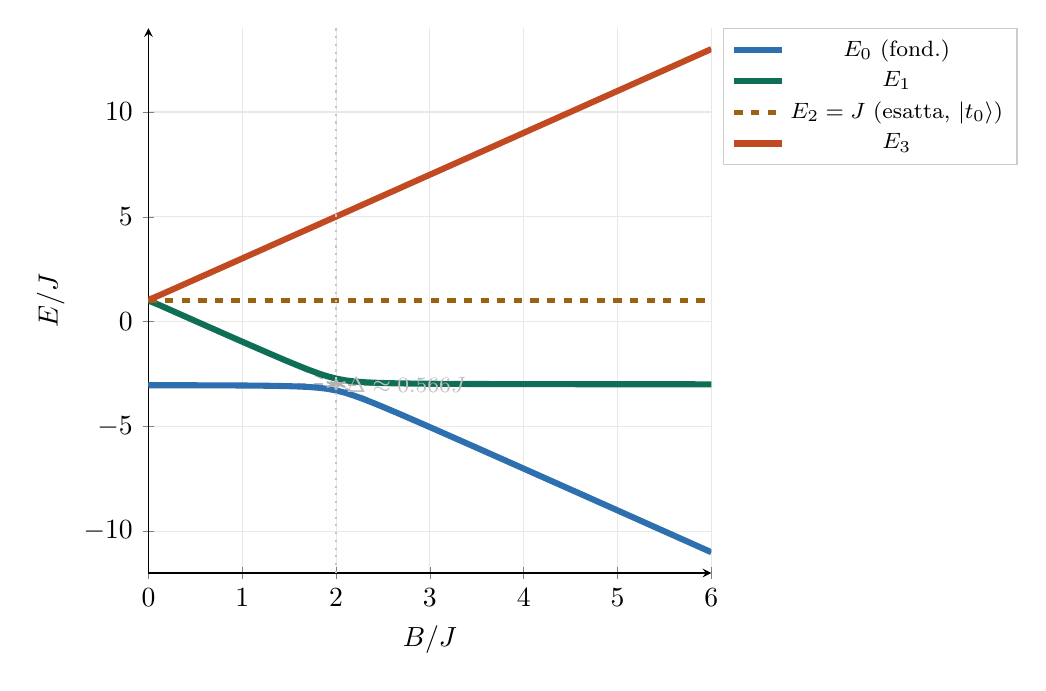
\begin{tikzpicture}
\begin{axis}[
  width=0.72\linewidth, height=8.5cm,
  xlabel={$B/J$}, ylabel={$E/J$},
  xmin=0, xmax=6, ymin=-12, ymax=14,
  axis lines=left, grid=both, grid style={gray!18},
  legend style={font=\footnotesize, at={(1.02,1)},
    anchor=north west, draw=gray!40, fill=white},
]
% --- D=0 reference (grey dashed) ---
\addplot[gray!55,dashed,thick,domain=0:6,samples=2,forget plot]{-3};
\addplot[gray!55,dashed,thick,domain=0:6,samples=2,forget plot]{1-2*x};
\addplot[gray!55,dashed,thick,domain=0:6,samples=2,forget plot]{1};
\addplot[gray!55,dashed,thick,domain=0:6,samples=2,forget plot]{1+2*x};

% --- E0 (fondamentale, con DM) ---
\addplot[spindown,line width=2.2pt] coordinates {
(0.00,-3.039608)(0.10,-3.039704)(0.20,-3.039996)(0.30,-3.040492)
(0.40,-3.041207)(0.50,-3.042163)(0.60,-3.043393)(0.70,-3.044939)
(0.80,-3.046862)(0.90,-3.049244)(1.00,-3.052201)(1.10,-3.055894)
(1.20,-3.060559)(1.30,-3.066550)(1.40,-3.074411)(1.50,-3.085023)
(1.60,-3.099862)(1.70,-3.121514)(1.80,-3.154572)(1.90,-3.206698)
(2.00,-3.287710)(2.10,-3.403132)(2.20,-3.548319)(2.30,-3.713491)
(2.40,-3.890661)(2.50,-4.074974)(2.60,-4.263692)(2.70,-4.455253)
(2.80,-4.648732)(2.90,-4.843557)(3.00,-5.039356)(3.10,-5.235883)
(3.20,-5.432966)(3.30,-5.630483)(3.40,-5.828344)(3.50,-6.026483)
(3.60,-6.224850)(3.70,-6.423405)(3.80,-6.622119)(3.90,-6.820965)
(4.00,-7.019926)(4.10,-7.218984)(4.20,-7.418127)(4.30,-7.617343)
(4.40,-7.816625)(4.50,-8.015963)(4.60,-8.215352)(4.70,-8.414786)
(4.80,-8.614260)(4.90,-8.813770)(5.00,-9.013313)(5.10,-9.212885)
(5.20,-9.412483)(5.30,-9.612106)(5.40,-9.811751)(5.50,-10.011416)
(5.60,-10.211100)(5.70,-10.410800)(5.80,-10.610517)(5.90,-10.810247)
(6.00,-11.009992)
}; \addlegendentry{$E_0$ (fond.)}

% --- E1 ---
\addplot[teal,line width=2.2pt] coordinates {
(0.00,1.000000)(0.10,0.819850)(0.20,0.621481)(0.30,0.422917)
(0.40,0.224426)(0.50,0.026087)(0.60,-0.172044)(0.70,-0.369913)
(0.80,-0.567451)(0.90,-0.764568)(1.00,-0.961147)(1.10,-1.157020)
(1.20,-1.351949)(1.30,-1.545577)(1.40,-1.737358)(1.50,-1.926409)
(1.60,-2.111252)(1.70,-2.289298)(1.80,-2.455955)(1.90,-2.603559)
(2.00,-2.722290)(2.10,-2.806624)(2.20,-2.861204)(2.30,-2.895811)
(2.40,-2.918429)(2.50,-2.933914)(2.60,-2.945003)(2.70,-2.953257)
(2.80,-2.959600)(2.90,-2.964605)(3.00,-2.968643)(3.10,-2.971959)
(3.20,-2.974725)(3.30,-2.977063)(3.40,-2.979062)(3.50,-2.980788)
(3.60,-2.982292)(3.70,-2.983611)(3.80,-2.984777)(3.90,-2.985813)
(4.00,-2.986740)(4.10,-2.987573)(4.20,-2.988324)(4.30,-2.989005)
(4.40,-2.989624)(4.50,-2.990190)(4.60,-2.990708)(4.70,-2.991183)
(4.80,-2.991622)(4.90,-2.992026)(5.00,-2.992401)(5.10,-2.992749)
(5.20,-2.993072)(5.30,-2.993373)(5.40,-2.993654)(5.50,-2.993917)
(5.60,-2.994163)(5.70,-2.994394)(5.80,-2.994611)(5.90,-2.994815)
(6.00,-2.995008)
}; \addlegendentry{$E_1$}

% --- E2 = J (t0, esatta) ---
\addplot[amber,dashed,line width=2.0pt] coordinates {
(0.00,1.000000)(6.00,1.000000)
}; \addlegendentry{$E_2=J$ (esatta, $\ket{t_0}$)}

% --- E3 ---
\addplot[spinup,line width=2.2pt] coordinates {
(0.00,1.039608)(0.10,1.219855)(0.20,1.418515)(0.30,1.617575)
(0.40,1.816781)(0.50,2.016076)(0.60,2.215437)(0.70,2.414852)
(0.80,2.614313)(0.90,2.813813)(1.00,3.013348)(1.10,3.212914)
(1.20,3.412508)(1.30,3.612127)(1.40,3.811769)(1.50,4.011432)
(1.60,4.211113)(1.70,4.410812)(1.80,4.610527)(1.90,4.810257)
(2.00,5.010000)(2.10,5.209756)(2.20,5.409523)(2.30,5.609302)
(2.40,5.809090)(2.50,6.008888)(2.60,6.208695)(2.70,6.408510)
(2.80,6.608332)(2.90,6.808162)(3.00,7.007999)(3.10,7.207842)
(3.20,7.407691)(3.30,7.607546)(3.40,7.807406)(3.50,8.007272)
(3.60,8.207142)(3.70,8.407017)(3.80,8.606896)(3.90,8.806779)
(4.00,9.006666)(4.10,9.206556)(4.20,9.406451)(4.30,9.606348)
(4.40,9.806249)(4.50,10.006153)(4.60,10.206060)(4.70,10.405969)
(4.80,10.605882)(4.90,10.805796)(5.00,11.005714)(5.10,11.205633)
(5.20,11.405555)(5.30,11.605479)(5.40,11.805405)(5.50,12.005333)
(5.60,12.205263)(5.70,12.405194)(5.80,12.605128)(5.90,12.805063)
(6.00,13.004999)
}; \addlegendentry{$E_3$}

% --- annotazione anti-incrocio ---
\draw[<->,gray!60,thick]
  (axis cs:2,-3.287710) -- (axis cs:2,-2.722290)
  node[midway,right,font=\footnotesize,gray!50]{$\Delta\approx0.566J$};
\draw[dotted,gray!45,thick]
  (axis cs:2,-12) -- (axis cs:2,14);
\end{axis}
\end{tikzpicture}
\caption{Spettro del dimero con campo $B$ e termine DM $D=0.2J$ (curve piene: autovalori
numerici esatti di~\eqref{eq:H4x4}) e caso $D=0$ (linee grigie tratteggiate). Il livello
$E_2=J$ (tratteggiato ambra) è l'autostato $t_0$, esatto per ogni $B,D$~\eqref{eq:Et0}.
A $B/J=2$ si apre l'anti-incrocio con gap
$\Delta=2\sqrt{2}\,D\approx0.566J$~\eqref{eq:gap}.}
\label{fig:spettro}
\end{figure}

\FloatBarrier
\section*{Tabella riassuntiva}

\begin{table}[htbp]
\centering
\renewcommand{\arraystretch}{1.4}
\begin{tabular}{llll}
\toprule
stato & $E$ (generale) & $E$ per $D\to0$ & $E$ per $b\to0$ \\
\midrule
$\ket{t_0}$ & $J$ (esatta, eq.~\eqref{eq:Et0}) & $J$ & $J$ \\
fondamentale
  & radice di~\eqref{eq:cubic}
  & $-3J$
  & $-J-2\sqrt{J^2+D^2}\approx-3J-\dfrac{D^2}{J}$ \\[6pt]
secondo livello
  & radice di~\eqref{eq:cubic}
  & $J-2b$
  & $J$ \\
terzo livello
  & radice di~\eqref{eq:cubic}
  & $J+2b$
  & $-J+2\sqrt{J^2+D^2}\approx J+\dfrac{D^2}{J}$ \\
\bottomrule
\end{tabular}
\caption{Riepilogo degli autovalori. Solo $\ket{t_0}$ ha forma chiusa per ogni $b,D$; gli altri tre
sono radici del cubico~\eqref{eq:cubic}.}
\label{tab:riepilogo}
\end{table}

\end{document}
